% =====================================================================
%  CHƯƠNG 3. MÔ HÌNH STEADYDET-N VÀ HUẤN LUYỆN NHẬN BIẾT RUNG
% =====================================================================
\chapter{Mô hình SteadyDet-N và phương pháp huấn luyện nhận biết rung}
\label{chap:mohinh}

Chương này trình bày mô hình phát hiện người do đề tài xây dựng. Phần đầu mô tả quá trình đi tới kiến trúc cuối cùng và lý do của từng lựa chọn; phần sau trình bày hàm mất mát, quy trình huấn luyện và phương pháp huấn luyện nhận biết rung, là đóng góp chính về mặt mô hình của đề tài.

\section{Yêu cầu thiết kế}

Mô hình phải thoả mãn đồng thời bốn yêu cầu, mỗi yêu cầu xuất phát từ một ràng buộc cụ thể của hệ thống:
\begin{enumerate}
\item \textbf{Phát hiện được người nhỏ}: khi máy bay lên cao hoặc người đi xa, bounding box chỉ còn vài chục điểm ảnh vuông, nên mô hình cần một mức dự đoán độ phân giải cao.
\item \textbf{Chi phí tính toán thấp}: một khung hình phải đi qua camera, mô hình, bộ theo vết và bộ điều khiển trong ngân sách 33,3\,ms của vòng lặp 30\,Hz trên một máy tính nhúng tản nhiệt thụ động.
\item \textbf{Chỉ dùng các phép toán mà NPU hỗ trợ}: mô hình phải biên dịch được bằng Hailo DFC và lượng tử hoá INT8 được.
\item \textbf{Bền trước rung}: độ chính xác phải giữ được khi ảnh bị nhoè và nhiễu do rung của khung máy bay.
\end{enumerate}

\section{Quá trình phát triển kiến trúc}

Kiến trúc được phát triển qua nhiều phiên bản, mỗi phiên bản được đo đạc trước khi quyết định hướng tiếp theo. Hai phiên bản quan trọng nhất được đặt tên trong báo cáo là \textbf{SteadyDet-W} (bản rộng) và \textbf{SteadyDet-N} (bản nano, bản cuối cùng). Trong mã nguồn, hai mô hình này tương ứng các tệp \texttt{pfdet\_nano\_v15.py} và \texttt{pfdet\_nano\_v17.py}.

SteadyDet-W đã có ít tham số (1,00 triệu) và chính xác nhất trong các phiên bản của nhóm, nhưng chi phí tính toán tới 12,9 GFLOPs ở độ phân giải 640. Phân tích chi phí theo từng lớp cho thấy nguyên nhân: riêng head ở mức $P_2$ ($160\times160$) đã tiêu tốn 1,82 GMACs, tức 28\% tổng chi phí, vì nó dùng năm lớp tích chập đầy đủ trên bản đồ lớn nhất. Đây là minh hoạ trực tiếp cho nhận xét ở Chương~\ref{chap:lythuyet}: số tham số ít không đồng nghĩa với chạy nhanh, vì chi phí tỷ lệ với diện tích feature map mà lớp đó xử lý. SteadyDet-N ra đời để giữ mức $P_2$ nhưng làm cho nó rẻ.

\section{Kiến trúc SteadyDet-N}
\label{sec:kientruc}

Hình~\ref{fig:kientruc} mô tả kiến trúc SteadyDet-N với cấu hình \textit{light} dùng trong toàn bộ đề tài. Mô hình có 1,17 triệu tham số và 4,6 GFLOPs với ảnh vào $640\times640$, là mô hình nhỏ nhất và rẻ nhất trong mọi bảng so sánh của báo cáo.

\begin{figure}[H]
\centering
\resizebox{0.97\textwidth}{!}{% Sơ đồ kiến trúc SteadyDet-N (profile light, ảnh vào 640x640)
\begin{tikzpicture}[
  font=\footnotesize, >={Stealth[length=2mm]},
  blk/.style={draw=black!60, rounded corners=2pt, align=center, minimum height=8.5mm, inner sep=2pt, fill=white},
  bb/.style={blk, fill=black!6, minimum width=3.3cm},
  nk/.style={blk, fill=xanh!10, minimum width=2.2cm},
  hd/.style={blk, fill=cam!12, minimum width=2.4cm},
  p2/.style={dashed, thick},
  lab/.style={font=\scriptsize, text=black!65}
]
% backbone
\node[blk, minimum width=3.3cm, fill=black!2] (in) at (0,0) {Ảnh vào\\$640\times640\times3$};
\node[bb, below=4mm of in] (stem) {EdgeContextStem\\$P_1$: $320^2$, 24 kênh};
\node[bb, below=4mm of stem, p2] (s2) {UIB (1 khối, bước 2)\\$P_2$: $160^2$, 48 kênh};
\node[bb, below=4mm of s2] (s3) {CSP-UIB (2 khối)\\$P_3$: $80^2$, 96 kênh};
\node[bb, below=4mm of s3] (s4) {CSP-UIB (2 khối)\\$P_4$: $40^2$, 144 kênh};
\node[bb, below=4mm of s4] (s5) {CSP-UIB (2 khối)\\$P_5$: $20^2$, 192 kênh};
\node[bb, below=4mm of s5, fill=xanh!22] (att) {Window self-attention\\(chỉ ở $P_5$)};
\foreach \a/\b in {in/stem,stem/s2,s2/s3,s3/s4,s4/s5,s5/att} \draw[->] (\a) -- (\b);

% neck (top-down)
\node[nk, right=2.3cm of att] (n5) {Conv $1\times1$\\48 kênh};
\node[nk, above=9.5mm of n5] (n4) {UIB\\48 kênh};
\node[nk, above=9.5mm of n4] (n3) {UIB\\48 kênh};
\node[nk, above=9.5mm of n3, p2] (n2) {UIB\\24 kênh};
\draw[->] (att) -- node[lab,above]{chiếu $1\times1$} (n5);
\draw[->] (s4.east) -- ++(0.9,0) |- (n4.west);
\draw[->] (s3.east) -- ++(0.7,0) |- (n3.west);
\draw[->] (s2.east) -- ++(0.5,0) |- (n2.west);
\draw[->, xanh, thick] (n5) -- node[lab,right]{$\uparrow2$, cộng} (n4);
\draw[->, xanh, thick] (n4) -- node[lab,right]{$\uparrow2$, cộng} (n3);
\draw[->, xanh, thick] (n3) -- node[lab,right]{$1\times1$, $\uparrow2$, cộng} (n2);

% heads
\node[hd, right=1.9cm of n2, p2] (h2) {LiteHead\\ra $160^2\times5$};
\node[hd, right=1.9cm of n3] (h3) {LiteHead\\ra $80^2\times5$};
\node[hd, right=1.9cm of n4] (h4) {LiteHead\\ra $40^2\times5$};
\node[hd, right=1.9cm of n5] (h5) {LiteHead\\ra $20^2\times5$};
\foreach \a/\b in {n2/h2,n3/h3,n4/h4,n5/h5} \draw[->] (\a) -- (\b);

\node[lab, above=1mm of s2.north east, anchor=south west, xshift=-4mm] {};
\node[font=\footnotesize\bfseries] at (0,1.0) {Backbone};
\node[font=\footnotesize\bfseries] at (n2 |- 0,1.0) {FPN neck (từ trên xuống)};
\node[font=\footnotesize\bfseries] at (h2 |- 0,1.0) {Head};
\node[draw=black!40, rounded corners=2pt, fill=black!3, align=left, font=\scriptsize, text width=3.9cm, below=6mm of h5] (lh)
 {\textbf{LiteHead:} DW $3\times3$ + PW $1\times1$ dùng chung $\rightarrow$ 1 kênh điểm người + 4 kênh hộp (hồi quy trực tiếp, không DFL).\\[2pt]
  Nét đứt: nhánh $P_2$ bước 4 được làm mỏng (1 khối, nửa số kênh neck, head depthwise separable).};
\end{tikzpicture}
}
\caption{Kiến trúc SteadyDet-N; độ phân giải giảm dần từ trên xuống. Chi phí được phân bổ không đối xứng: nhánh $P_2$ (nét đứt) chỉ có một khối, số kênh bằng một nửa và head tách được, còn các khối CSP hai tầng và phép self-attention nằm ở những mức có bản đồ nhỏ}
\label{fig:kientruc}
\end{figure}

\subsection{Backbone}

\textbf{Khối đầu vào EdgeContextStem.} Ảnh vào được xử lý song song bởi hai nhánh: nhánh cục bộ gồm hai tích chập $3\times3$ (lớp đầu có bước 2) giữ chi tiết cạnh, và nhánh ngữ cảnh gồm phép lấy trung bình $2\times2$ rồi một tích chập $3\times3$. Hai nhánh được ghép kênh và trộn bằng tích chập $1\times1$, cho ra bản đồ $P_1$ kích thước $320\times320$ với 24 kênh. Việc giảm độ phân giải bằng hai con đường bổ trợ giúp giữ thông tin của các vật rất nhỏ ngay từ lớp đầu tiên.

\textbf{Mức $P_2$ chỉ một khối.} Mức bước 4 dùng đúng một khối UIB~\cite{qin2024mnv4} có bước 2, gồm tích chập depthwise $3\times3$, mở rộng kênh $1\times1$ với hệ số 4, rồi thu hẹp $1\times1$ về 48 kênh. SteadyDet-W dùng ba khối ở mức này; giảm xuống một khối cắt phần lớn chi phí của mức đắt nhất.

\textbf{Các mức $P_3$--$P_5$.} Ba mức sâu hơn dùng khối CSP-UIB: một khối UIB giảm mẫu, sau đó bản đồ được tách thành hai nửa theo kênh, một nửa đi qua hai khối UIB, nửa kia đi tắt, rồi hai nửa được ghép lại và trộn bằng tích chập $1\times1$ theo ý tưởng của CSPNet~\cite{wang2020cspnet}. Số kênh lần lượt là 96, 144 và 192. Ở $P_3$ và $P_4$, khối UIB có thêm một tích chập depthwise để mở rộng receptive field với chi phí thấp. Chi phí tính toán được dồn vào các mức này vì bản đồ ở đây nhỏ: $80\times80$, $40\times40$ và $20\times20$.

\textbf{Self-attention chỉ ở $P_5$.} Sau mức $P_5$, một khối self-attention theo cửa sổ~\cite{liu2021swin} với window size 3 và 2 attention head cho mô hình ngữ cảnh toàn cục (ví dụ phân biệt người với cột điện hay bóng đổ). Đặt ở $20\times20$ nên chi phí của nó không đáng kể.

\subsection{FPN neck mỏng}

Neck của mạng là một FPN~\cite{lin2017fpn} chỉ có đường từ trên xuống. Mỗi mức của backbone được chiếu về số kênh chung bằng tích chập $1\times1$: 48 kênh cho $P_3$--$P_5$ và chỉ \textbf{24 kênh cho $P_2$}. Bản đồ mức trên được phóng to gấp đôi bằng nội suy nearest-neighbor, cộng với bản đồ mức dưới, rồi đi qua một khối UIB. Riêng khi đi từ $P_3$ xuống $P_2$, bản đồ được chiếu từ 48 về 24 kênh trước khi phóng to. Việc giảm một nửa số kênh ở mức $160\times160$ làm chi phí mọi lớp ở mức này giảm khoảng bốn lần.

\subsection{Head LiteHead}

Mỗi mức có một head LiteHead gồm một tích chập depthwise $3\times3$ và một tích chập $1\times1$ dùng chung, sau đó tách thành hai tích chập $1\times1$: một cho điểm có người (1 kênh), một cho bounding box (4 kênh). Như vậy mỗi head xuất một tensor $5 \times H \times W$ ở bốn bước 4, 8, 16 và 32. So với head tách rời năm lớp tích chập đầy đủ của SteadyDet-W, LiteHead rẻ hơn nhiều mà vẫn tách hai nhiệm vụ phân loại và hồi quy. Hộp được hồi quy trực tiếp (không dùng phân phối rời rạc), tương tự hướng của YOLO26~\cite{ultralytics}. Độ lệch ban đầu của kênh phân loại được đặt bằng $-5{,}5$ để xác suất ban đầu xấp xỉ 0,004, tránh việc hàng chục nghìn ô nền sinh hộp sai trong những epoch đầu.

\textbf{Giải mã.} Với grid cell $(i, j)$ ở bước $s$ và đầu ra $(t_x, t_y, t_w, t_h)$, hộp dự đoán được giải mã như sau:
\begin{equation}
c_x = \big(j + \mathrm{sigmoid}(t_x) - 0{,}5\big)\, s, \quad
c_y = \big(i + \mathrm{sigmoid}(t_y) - 0{,}5\big)\, s, \quad
w = e^{t_w} s, \quad h = e^{t_h} s.
\label{eq:decode}
\end{equation}
Mọi phép toán của mô hình (tích chập, batch norm được gộp vào tích chập, SiLU, cộng, ghép kênh, nội suy) đều được Hailo DFC hỗ trợ, trừ khối self-attention; Chương~\ref{chap:trienkhai} trình bày cách xử lý khối này khi triển khai.

\subsection{So sánh hai phiên bản}

\begin{table}[H]
\centering
\caption{So sánh cấu trúc và chi phí của SteadyDet-W và SteadyDet-N (ảnh vào $640\times640$)}
\label{tab:sosanhkientruc}
\small
\renewcommand{\arraystretch}{1.15}
\begin{tabularx}{\textwidth}{@{}l>{\centering\arraybackslash}X>{\centering\arraybackslash}X@{}}
\toprule
\textbf{Thành phần} & \textbf{SteadyDet-W} & \textbf{SteadyDet-N}\\
\midrule
Số khối ở mức $P_2$ & 3 & 1\\
Số kênh cổ ở mức $P_2$ & bằng các mức khác & một nửa (24)\\
Head & tách rời 5 tích chập đầy đủ & LiteHead depthwise separable\\
Vị trí self-attention & $P_4$ và $P_5$ & chỉ $P_5$\\
Số tham số & 1,00 triệu & 1,17 triệu\\
Chi phí tính toán & 12,9 GFLOPs & \textbf{4,6 GFLOPs} (giảm 2,8 lần)\\
\bottomrule
\end{tabularx}
\end{table}

SteadyDet-N có nhiều tham số hơn SteadyDet-W một chút vì phần tính toán được dồn về các mức sâu, nơi số kênh lớn; nhưng chính các mức này có bản đồ nhỏ nên tổng chi phí giảm 2,8 lần.

\section{Hàm mất mát}
\label{sec:hammatmat}

Tổng hàm mất mát gồm hai thành phần:
\begin{equation}
\mathcal{L}_{\det} = \lambda_{\text{obj}}(e)\, \mathcal{L}_{\text{obj}} + \lambda_{\text{box}}(e)\, \mathcal{L}_{\text{box}},
\end{equation}
trong đó $e$ là chỉ số epoch.

\textbf{Thành phần phân loại} $\mathcal{L}_{\text{obj}}$ là hàm QFL~\cite{li2020gfl} theo phương trình~(\ref{eq:qfl}) với $\beta = 2$, nhãn mềm là IoU giữa hộp dự đoán và hộp thật tại các ô dương.

\textbf{Thành phần hồi quy} kết hợp NWD và CIoU với trọng số phụ thuộc diện tích hộp thật $A$ (điểm ảnh vuông):
\begin{equation}
\mathcal{L}_{\text{box}} = w_{\text{ASL}}(A)\Big[\, \omega(A)\,\big(1 - \mathrm{NWD}\big) + \big(1 - \omega(A)\big)\,\mathcal{L}_{\mathrm{CIoU}} \Big],
\qquad \omega(A) = \exp\!\left(-\frac{A}{1024}\right).
\label{eq:boxloss}
\end{equation}
Với người rất nhỏ ($A \ll 32^2$), $\omega \approx 1$ và NWD chiếm ưu thế nhờ gradient ổn định; với người lớn, CIoU chiếm ưu thế vì nó phạt chính xác hình dạng hộp. Hằng số chuẩn hoá NWD là $C = 0{,}019$ theo toạ độ chuẩn hoá. Hệ số $w_{\text{ASL}}(A) = \mathrm{clip}\big(\sqrt{A_{\text{ref}}/A},\, 1,\, 4\big)$ tăng trọng số cho vật nhỏ, với $A_{\text{ref}}$ tương ứng 0,4\% diện tích ảnh.

\textbf{Gán nhãn nhận biết mục tiêu nhỏ.} Việc chọn ô dương dựa trên mức độ phù hợp theo TOOD~\cite{feng2021tood}, $t = s^{\alpha}\cdot \mathrm{IoU}^{\beta}$ với $\alpha = 1$, $\beta = 8$. Vì một người nhỏ chỉ phủ vài grid cell, chiến lược mặc định dễ cấp cho họ quá ít ô dương. Đề tài áp dụng hai điều chỉnh: người có diện tích dưới 576 điểm ảnh vuông ($24^2$) được cấp tới 6 ô dương và vùng tìm kiếm bán kính 3 ô, còn người lớn hơn được cấp 3 ô với bán kính 2; đồng thời số ô dương tối thiểu cho mục tiêu nhỏ không dưới 4.

\textbf{Cân bằng tiến triển.} Ở đầu quá trình huấn luyện, mô hình cần học ``có người hay không'' trước khi học ``hộp khít tới đâu''. Trọng số hai thành phần được nội suy tuyến tính theo tiến độ huấn luyện: $\lambda_{\text{obj}}$ giảm từ $2\times8$ về 8 và $\lambda_{\text{box}}$ tăng từ $4/2$ lên 4.

\section{Quy trình huấn luyện}
\label{sec:quytrinhhuanluyen}

\textbf{Bộ tối ưu.} Đề tài dùng MuSGD, bộ tối ưu lai được Ultralytics giới thiệu cùng YOLO26~\cite{ultralytics}, kết hợp Muon~\cite{jordan2024muon} với SGD có quán tính Nesterov. Với các tensor trọng số nhiều chiều, bước cập nhật là tổng của hai phần: phần Muon (hệ số 0,2), trong đó gradient được trực giao hoá xấp xỉ bằng 5 vòng lặp Newton--Schulz, và phần SGD (hệ số 1,0); các tham số một chiều (độ lệch, batch norm) chỉ dùng SGD. Trong các thử nghiệm của nhóm trên SteadyDet-W, MuSGD cho AP@0,5 kiểm định 0,5932, cao nhất trong các bộ tối ưu đã thử.

\textbf{Huấn luyện gốc (nhánh chuẩn).} SteadyDet-N được huấn luyện từ khởi tạo ngẫu nhiên trong 300 epoch, batch size 16 với tích luỹ gradient 6 bước, learning rate 0,01 giảm theo hàm cosin xuống $10^{-4}$, 10 epoch warm-up, weight decay $5\times10^{-4}$, huấn luyện độ chính xác hỗn hợp và EMA của trọng số với hệ số 0,9998. Phép ghép bốn ảnh được tắt trong 60 epoch cuối. Mô hình được đánh giá trên tập kiểm định sau mỗi 5 epoch.

\textbf{Nhánh triển khai.} Mô hình được huấn luyện 400 epoch với batch size 12; dữ liệu COCO-person được trộn với tỷ lệ 25\% từ epoch 100 tới epoch 360. Khi cần triển khai lên NPU, mô hình này được tinh chỉnh thêm 20 epoch với learning rate $10^{-3}$ ở cấu hình không có khối self-attention (Chương~\ref{chap:trienkhai}).

\begin{figure}[H]
\centering
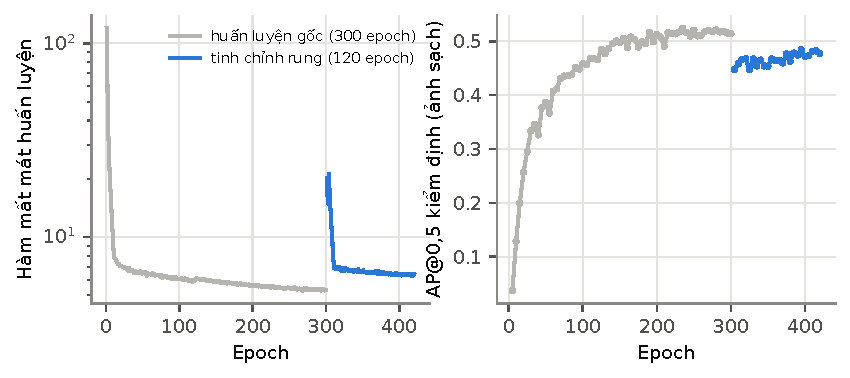
\includegraphics[width=\textwidth]{huan_luyen.pdf}
\caption{Hàm mất mát huấn luyện (trái, thang log) và AP@0,5 trên tập kiểm định ảnh sạch (phải) của SteadyDet-N nhánh chuẩn: 300 epoch huấn luyện gốc (xám) và 120 epoch tinh chỉnh nhận biết rung (xanh). Hàm mất mát tăng vọt khi bắt đầu tinh chỉnh vì một nửa số lô là ảnh đã bị làm rung}
\label{fig:huanluyen}
\end{figure}

\section{Huấn luyện nhận biết rung}
\label{sec:huanluyenrung}

\subsection{Ý tưởng}

Nguyên nhân gốc khiến bộ phát hiện sụp đổ khi rung là \textit{sai lệch phân phối}: VisDrone được thu từ các nền tảng ổn định, nên mô hình chưa bao giờ thấy ảnh nhoè do rung trong huấn luyện nhưng lại gặp nó liên tục khi bay. Các phép tăng cường chuẩn ở Chương~\ref{chap:dulieu} như lật ảnh, co giãn hay đổi màu chỉ lấy mẫu những biến đổi mà dữ liệu vốn đã chứa; chúng không sinh ra loại suy giảm này. Phương pháp của đề tài vì thế rất trực tiếp: đưa chính toán tử rung vào phân phối huấn luyện.

\subsection{Phương pháp}

Gọi $\mathcal{T}$ là toán tử rung ngẫu nhiên của giao thức VisDrone-Shake (mục~\ref{sec:shake}), trong đó mức rung được chọn ngẫu nhiên đều trong $\{1, 2, 3\}$ và hướng nhoè được rút lại cho mỗi batch. Trong huấn luyện, mỗi batch $x$ được thay bằng $\mathcal{T}(x)$ với xác suất $p = 0{,}5$, và hàm mất mát phát hiện thông thường được tính trên ảnh mà mạng nhận được:
\begin{equation}
\mathcal{L} = \mathcal{L}_{\det}\big(f_\theta(\hat{x}),\, y\big), \qquad
\hat{x} =
\begin{cases}
\mathcal{T}(x) & \text{với xác suất } p,\\
x & \text{ngược lại}.
\end{cases}
\label{eq:vibaware}
\end{equation}
Vì $\mathcal{T}$ không làm dịch chuyển đối tượng, nhãn $y$ không cần điều chỉnh; đây chính là điều làm cho phép thay thế hợp lệ. Phương pháp không thêm mô-đun nào, không cần truyền xuôi hai lần, và mô hình xuất ra để triển khai có cấu trúc giống hệt mô hình gốc, nên \textbf{chi phí suy luận không thay đổi}. Chi phí huấn luyện tăng thêm chỉ là một phép tích chập depthwise và hai phép toán từng phần tử trên GPU. Hình~\ref{fig:huanluyenrung}(a) minh hoạ phương pháp.

\begin{figure}[H]
\centering
\resizebox{\textwidth}{!}{% Sơ đồ huấn luyện nhận biết rung (trên) và biến thể ràng buộc nhất quán (dưới)
\begin{tikzpicture}[
  font=\footnotesize, >={Stealth[length=2mm]},
  box/.style={draw=black!60, rounded corners=2pt, align=center, minimum height=9mm, inner sep=3pt, fill=white},
  op/.style={box, fill=cam!14},
  net/.style={box, fill=xanh!14, minimum width=2.1cm},
  loss/.style={box, fill=black!7},
  dec/.style={diamond, draw=black!60, aspect=2.2, inner sep=1pt, align=center, fill=white, font=\scriptsize}
]
\node[font=\footnotesize\bfseries, anchor=west] at (-0.4,1.1) {(a) Huấn luyện nhận biết rung (phương pháp đề xuất)};
\node[box] (x) at (0,0) {Lô ảnh $x$\\+ nhãn $y$};
\node[dec, right=6mm of x] (d) {xác suất\\$p=0{,}5$};
\node[op, right=7mm of d] (T) {Toán tử rung $\mathcal{T}$\\nhoè $L,\theta$ + nhiễu $\sigma$ + sáng $b$};
\node[net, right=7mm of T] (f) {Mạng\\$f_\theta$};
\node[loss, right=7mm of f] (L) {$\mathcal{L}_{\det}\big(f_\theta(\hat{x}), y\big)$\\nhãn giữ nguyên};
\draw[->] (x) -- (d);
\draw[->] (d) -- node[above,font=\scriptsize]{có} (T);
\draw[->] (T) -- node[above,font=\scriptsize]{$\hat x$} (f);
\draw[->] (d.south) -- ++(0,-0.55) -| node[pos=0.25,below,font=\scriptsize]{không: $\hat x = x$} (f.south);
\draw[->] (f) -- (L);

\begin{scope}[yshift=-3.75cm]
\node[font=\footnotesize\bfseries, anchor=west] at (-0.4,1.5) {(b) Biến thể ràng buộc nhất quán (đối chứng, cho kết quả kém hơn)};
\node[box] (x2) at (0,0) {Lô ảnh $x$\\+ nhãn $y$};
\node[net] (fc) at (4.2,0.75) {$f_\theta(x)$ nhánh sạch};
\node[op] (T2) at (2.0,-0.75) {$\mathcal{T}$};
\node[net] (fv) at (4.2,-0.75) {$f_\theta(\tilde x)$ nhánh rung};
\node[loss, anchor=west] (Ld) at (7.4,0.75) {$\mathcal{L}_{\det}(f_\theta(x), y)$};
\node[loss, anchor=west] (sg) at (7.4,-0.75) {$\lambda\,\mathcal{L}_{\text{cons}}\big(f_\theta(\tilde x),\ \mathrm{sg}[f_\theta(x)]\big)$};
\draw[->] (x2.east) -- ++(0.35,0) |- (fc.west);
\draw[->] (x2.east) -- ++(0.35,0) |- (T2.west);
\draw[->] (T2) -- node[above,font=\scriptsize]{$\tilde x$} (fv);
\draw[->] (fc) -- (Ld);
\draw[->] (fv) -- (sg);
\draw[->, dashed] (fc.east) ++(0.2,0) -- node[left,font=\scriptsize, pos=0.5]{dừng gradient} ($(sg.north west)+(0.4,0)$);
\end{scope}
\end{tikzpicture}
}
\caption{(a) Huấn luyện nhận biết rung: một nửa số lô được thay bằng bản đã làm rung và tính hàm mất mát phát hiện thông thường. (b) Biến thể ràng buộc nhất quán: truyền xuôi cả hai bản và kéo dự đoán trên ảnh rung về phía dự đoán trên ảnh sạch đã dừng gradient. Cả hai chỉ tồn tại khi huấn luyện}
\label{fig:huanluyenrung}
\end{figure}

\subsection{Biến thể ràng buộc nhất quán}

Trước khi có kết quả, nhóm kỳ vọng rằng có thể khai thác nhiều tín hiệu hơn từ ảnh rung so với chỉ dùng nhãn. Biến thể này, lấy cảm hứng từ các phương pháp học bán giám sát dựa trên tính nhất quán, truyền cả $x$ và $\tilde{x} = \mathcal{T}(x)$ qua cùng một mạng, tính hàm mất mát phát hiện trên nhánh sạch, và thêm một thành phần kéo dự đoán trên ảnh rung về phía bản sao đã dừng gradient của dự đoán sạch:
\begin{equation}
\mathcal{L} = \mathcal{L}_{\det}\big(f_\theta(x), y\big) + \lambda\, \mathcal{L}_{\text{cons}}\Big(f_\theta(\tilde{x}),\ \mathrm{sg}\big[f_\theta(x)\big]\Big), \qquad \lambda = 0{,}5.
\label{eq:vibcons}
\end{equation}
$\mathcal{L}_{\text{cons}}$ gồm ba phần cộng trên các mức: entropy chéo có nhiệt độ $T = 2$ giữa điểm tin cậy hai nhánh, sai số $L_1$ trơn trên toạ độ hộp chỉ tại các ô mà nhánh sạch tin cậy trên 0,1, và sai số bình phương giữa đặc trưng cổ mạng với trọng số 0,5. Phép dừng gradient là bắt buộc: nếu thiếu nó, cách dễ nhất để giảm $\mathcal{L}_{\text{cons}}$ là làm dự đoán sạch kém đi cho giống dự đoán rung, tức phá huỷ bộ phát hiện. Biến thể này cần hai lượt truyền xuôi nên tốn khoảng 1,8 lần thời gian huấn luyện. Chương~\ref{chap:ketqua} cho thấy nó thực tế kém hơn phương pháp đơn giản.

\subsection{Thiết lập tinh chỉnh}

Huấn luyện nhận biết rung được áp dụng như một giai đoạn \textit{tinh chỉnh}: xuất phát từ checkpoint tốt nhất của huấn luyện gốc, tinh chỉnh 120 epoch với batch size 8 và tích luỹ gradient 12 bước, MuSGD với learning rate $2\times10^{-3}$, 3 epoch warm-up trước khi bật toán tử rung. Nhờ vậy phương pháp có thể áp dụng cho một mô hình đã huấn luyện xong mà không phải lặp lại toàn bộ lịch trình. Checkpoint được chọn theo AP kiểm định trên ảnh sạch, đúng quy tắc áp dụng cho mô hình gốc.

Để tách bạch tác dụng của rung khỏi tác dụng của việc huấn luyện thêm 120 epoch, đề tài chạy một \textbf{thí nghiệm đối chứng}: tinh chỉnh mô hình gốc đúng 120 epoch với cùng mọi siêu tham số nhưng tắt toán tử rung. Cả ba cấu hình (đối chứng, nhận biết rung, ràng buộc nhất quán) chỉ khác nhau đúng một biến.

\subsection{Biến thể không dùng NMS}

Đề tài cũng thử một biến thể SteadyDet-N không cần NMS theo ý tưởng của YOLOv10~\cite{wang2024yolov10}: thêm một head LiteHead ``one-to-one'' song song dùng chung đặc trưng, huấn luyện đồng thời với head ``one-to-many'', và khi suy luận chỉ dùng head one-to-one. Biến thể này đạt AP@[.50:.95] 0,1954 trên ảnh sạch và retain 23,4 $\pm$ 0,8\%. Tuy nhiên, trên hệ thống thực tế NMS chỉ tốn trung vị 0,84\,ms mỗi khung (Chương~\ref{chap:trienkhai}), nên việc bỏ NMS không mang lại lợi ích đáng kể về độ trễ; đề tài giữ head thông thường cho các thí nghiệm chính và triển khai.

\section{Kết luận chương}

SteadyDet-N giữ mức dự đoán bước 4 cho người nhỏ nhưng làm nhánh này mỏng đi, dồn tính toán về các mức sâu, dùng head depthwise separable, nhờ đó giảm chi phí 2,8 lần so với SteadyDet-W xuống 4,6 GFLOPs với 1,17 triệu tham số. Hàm mất mát kết hợp QFL, NWD và CIoU theo diện tích cùng chiến lược gán nhãn ưu tiên mục tiêu nhỏ. Phương pháp huấn luyện nhận biết rung đưa mô hình vật lý của rung vào phân phối huấn luyện, không đổi nhãn, không đổi mô hình khi suy luận. Chương tiếp theo kiểm chứng các thiết kế này bằng thực nghiệm có đối chứng.
